\begin{lemma}[\textbf{Cut Lemma}]
Let $X \subseteq E$ be a good set. If $(V, X)$ is not a spanning tree, then $(V, X)$ consists of two or more connected components. Let $V = S \cup \overline{S}$ be a cut of $X$. That is, no edge of $X$ goes from $S$ to $\overline{S}$. Let $e \in E$ be an edge of minimum cost connecting two connecting components of $(V, X)$. Then $X \cup \{e\}$ is good, too.
\end{lemma}
\begin{proof}
Suppose the $X \cup \{e\}$ is not a good set. Then all of the minimum spanning trees exclude the minimum edge which connects the two connecting components of $(V, X)$. Denote these two connecting components as $C_1$ and $C_2$. According to the property of spanning tree, for each minimum spanning tree $T_m$, there is exactly one edge connecting $C_1$ and $C_2$ which we denote as $e_t\in E(T_m)$. Substitute $e_t$ to $e_m$ and obvirusly the new spanning tree is still a spanning tree $T'_m$. And using the following argumentation, we get a smaller spanning tree.
\begin{figure}[H]
	\centering
	\subfigure[Original minimum spanning tree]{
	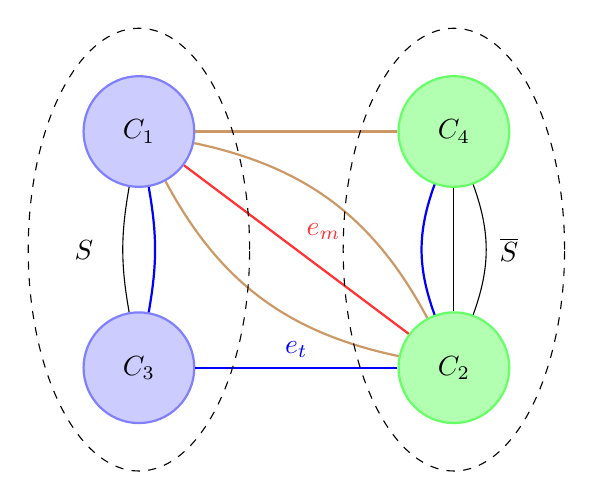
\begin{tikzpicture}
		[place1/.style={circle,draw=blue!50,fill=blue!20,thick,
inner sep=0pt,minimum size=40pt},
		place2/.style={circle,draw=green!60,fill=green!30,thick,
inner sep=0pt,minimum size=40pt},
		textstyle/.style={},
		bend angle=45,
		edgestyle/.style={-,shorten <=1pt,>=stealth’,semithick}]
		\node at (-2.0, 1.5) (one) [place1] {$C_1$};
		\node at (-2.0, -1.5) (three) [place1] {$C_3$}
			edge [-,bend left=10] (one)
			edge [-,bend right=10,blue!100,thick] (one);
		\node at (2.0, -1.5) (two) [place2] {$C_2$}
			edge [-,bend left=25,brown!80,thick] (one)
			edge [-,bend left=0,red!80,thick] node[auto,swap] {$e_m$} (one)
			edge [-,bend right=25,brown!80,thick] (one)
			edge [-,bend right=0,blue!100,thick] node[auto,swap] {$e_t$} (three);
		\node at (2.0, 1.5) (four) [place2] {$C_4$}
			edge [-,bend right=20,blue!100,thick] (two)
			edge [-,bend right=0] (two)
			edge [-,bend left=20] (two)
			edge [-,bend right=0,brown!80,thick] (one);
		\node at (-2.7, 0) (text1) [textstyle] {$S$};
		\node at (2.7, 0) (text2) [textstyle] {$\overline{S}$};
		\draw[dashed] (-2.0, 0) ellipse [x radius=40pt, y radius=80pt];
		\draw[dashed] (2.0, 0) ellipse [x radius=40pt, y radius=80pt];
	\end{tikzpicture}
	}
	\subfigure[Generated spanning tree]{
	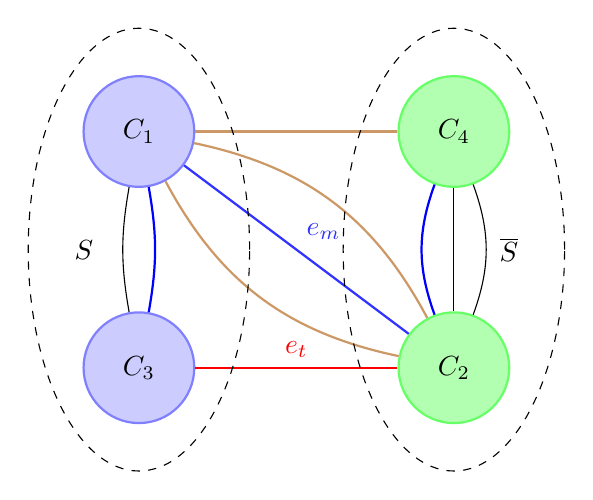
\begin{tikzpicture}
		[place1/.style={circle,draw=blue!50,fill=blue!20,thick,
inner sep=0pt,minimum size=40pt},
		place2/.style={circle,draw=green!60,fill=green!30,thick,
inner sep=0pt,minimum size=40pt},
		textstyle/.style={},
		bend angle=45,
		edgestyle/.style={-,shorten <=1pt,>=stealth’,semithick}]
		\node at (-2.0, 1.5) (one) [place1] {$C_1$};
		\node at (-2.0, -1.5) (three) [place1] {$C_3$}
			edge [-,bend left=10] (one)
			edge [-,bend right=10,blue!100,thick] (one);
		\node at (2.0, -1.5) (two) [place2] {$C_2$}
			edge [-,bend left=25,brown!80,thick] (one)
			edge [-,bend left=0,blue!80,thick] node[auto,swap] {$e_m$} (one)
			edge [-,bend right=25,brown!80,thick] (one)
			edge [-,bend right=0,red!100,thick] node[auto,swap] {$e_t$} (three);
		\node at (2.0, 1.5) (four) [place2] {$C_4$}
			edge [-,bend right=20,blue!100,thick] (two)
			edge [-,bend right=0] (two)
			edge [-,bend left=20] (two)
			edge [-,bend right=0,brown!80,thick] (one);
		\node at (-2.7, 0) (text1) [textstyle] {$S$};
		\node at (2.7, 0) (text2) [textstyle] {$\overline{S}$};
		\draw[dashed] (-2.0, 0) ellipse [x radius=40pt, y radius=80pt];
		\draw[dashed] (2.0, 0) ellipse [x radius=40pt, y radius=80pt];
	\end{tikzpicture}
	}
	\caption{The illustration of the proof}
\end{figure}
The ``costs'' of the new spanning tree $T'_m$ is:
\[c(T'_m) = \sum_{e \in E(T')}c(e) = c(T_m) - c(e_t) + c(e_m)\]
Using the condition $e_m$ is the minimum edge connecting $C_1$ and $C_2$, we can easily know that:
\[c(e_m) \leq c(e_t)\]
Then we obtain a more optimal spanning tree(or we obtain another minimum spanning tree containing the edge $e_m$) which leads the contradictory according to the inequality below:
\[c(T'_m) = c(T_m) - c(e_t) + c(e_m) \leq c(T_m)\]
Hence, $X \cup \{e\}$ is good.
\end{proof}
\begin{lemma}[\textbf{The Inverse of Cut Lemma}]
If $X$ is good, $e \notin X$, and $X \cup \{e\}$ is good, then there is a cut $S$, $V \backslash S$ such that the following two holds:
\begin{spacing}{0.6}
\begin{enumerate}
\item no edge from $X$ crosses this cut;
\item $e$ is minimum weight edge of $G$ crossing the cut.
\end{enumerate}
\end{spacing}
\end{lemma}
